\documentclass[../main.tex]{subfiles}
\graphicspath{ {images/Images/} }
\begin{document}

Como se dijo previamente, las redes neuronales de convolución hacen parte de las redes neuronales, así que para ser más claros se hablará primero acerca de redes neuronales artificiales para después pasar a las de convolución. Es importante tener en cuenta que la siguiente sección hablará acerca de algo que en las redes de convolución se conoce como capas completamente conectadas. \\

\section{Estructura de la red neuronal artificial}

\subsection{Neurona}

Siguiendo el principio de las redes neuronales biológicas, el algoritmo que se desarrolla está organizado jerárquicamente donde las respuestas obtenidas por muchas neuronas se convierten en los parámetros de entrada de las siguientes. Además, la red neuronal artificial será al fin y al cabo una conexión de capas de neuronas. A cada una de las neuronas se le asigna una suma de las entradas con un peso dado que luego será evaluado dentro de la función de activación, y posteriormente se genera el valor de salida[vanderBaan]. El propósito de esos pesos se observa cuando el proceso de aprendizaje empieza, ya que son parámetros que varían en busca de la optimización del código. \\  

\subsection{Función de activación}
Como se mencionó, existe una función de activación que recibe ciertas características como parámetro, donde dependiendo de la función puede que el resultado se vea reflejado como una activación de la neurona. Es decir, dependiendo de la entrada que reciba puede que la función entregue un parámetro binario que se pueda expresar como un filtro de la señal de entrada. La función que se usa más comúnmente es una función sigmoidea de la forma[Thomas, libro]: 

\begin{equation}
    f(x) = \frac{1}{1+e^{-x}}
\end{equation}

\noindent
A veces puede considerarse una función tipo "heavyside" o escalón que sirva como función de activación para la neurona, ya que tiene una pendiente más marcada que defina el punto de activación[Thomas].  \\


\subsection{Bias o sesgo} 

El sesgo es un parámetro que se usa cuando se busca resaltar la flexibilidad de la neurona, ya que permite ajustar el valor de x para el cual la función de activación se activa, valga la redundancia. A diferencia del sesgo, los pesos que se le dan a cada nodo dentro de las capas alteran la pendiente de la función de activación. 

\subsection{Red completa}
En la figura 3.1 podemos observar un esquema de una red neuronal artificial compuesta de tres capas. Es un caso simple que ayuda a entender como se conectan las partes mencionadas anteriormente. 

\begin{figure}[h]
    \centering
    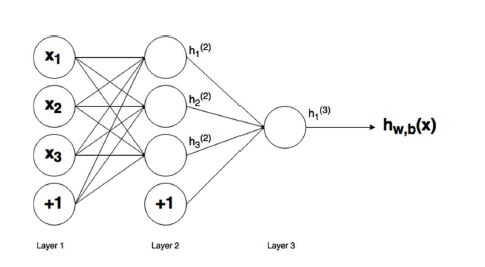
\includegraphics[width=0.7\textwidth]{ANN.JPG}
    \label{fig:ejemplo}
    \centering
    \caption{\centering Esquema de una red neuronal de 3 capas. La capa 1 representa los valores de entrada de la red, la capa 2 contiene la suma ponderada y la función de activación, y la capa 3 representa los valores de salida. Las capas están compuestas de neuronas, las cuales se representan mediante circulos. Tomada de (Thomas)}
\end{figure}

Es importante notar que la capa dos es la más importante en este caso y usualmente se le llama capa oculta porque no representa ni la entrada ni la salida de la red. De manera breve podemos resumir el proceso de las redes neuronales artificiales. Primero, decimos que cada valor de entrada (representado con $X_i$) está conectado a cada neurona en la siguiente capa. Esto es algo que en las redes neuronales de convolución llaman capas completamente conectadas. Cada Neurona en la capa dos recibe cada uno de los elementos de entrada, les asigna un peso y los suma. Luego le suma un elemento de bias, representado en la imagen como +1. El resultado de esta suma se opera en la función de activación y su resultado (notado en el esquema como $h_i^{2}$) se evalúa nuevamente en la función de activación para obtener el resultado final de la clasificación. 
 
\newpage
\section{Detección automática de ondas sísmicas}

Durante los últimos años, se ha puesto un gran esfuerzo en diseñar algoritmos capaces de detectar llegadas de ondas sismológicas P y S de manera automática. Entre estos métodos se destaca el de promedio de tiempos cortos(STA) y de tiempos largos(LTA) de la señal, así como métodos autoregresivos, algoritmos basados en la polarización de la onda (bueno para distinguir entre ondas P y S(Zhu)), y redes neuronales. Así que primero hablaremos un poco de los métodos alternativos a las redes neuronales para después enfocarnos en las redes neuronales.\\

El método de STA/LTA calcula la relación de la energía promedio de tiempos largos y cortos para varios receptores. Si un evento es detectado por un mínimo de 4 estaciones, entonces de considera una llegada de onda (Wu). Es un método eficiente, generalmente efectivo, pero susceptible al ruido y con baja precisión para ondas de cizalla. (Zhu) Por su parte Fischer, et al. propuso un método de detección automática de ondas P-S para un arreglo lineal de receptores, como en un borehole usado en un reservorio de hidrocarburos. La técnica de ellos consistía en usar el carácter dominante de ondas S directas en configuraciones microsísmicas. Por lo tanto, las ondas S se detectaban buscando el máximo de la energía polarizada con el máximo del promedio de tiempos cortos sobre el promedio de tiempos largos. Otro autor que optó por el método de STA/LTA para la detección de ondas sismológicas fue Ross (2014) donde presentó un algoritmo basado en curtosis, oblicuidad y STA/LTA.\\


Las redes neuronales fueron los primeros métodos de machine learning usados para la detección de ondas sismológicas. Las capas conectadas completamente, como usualmente son, requieren de una buena optimización para poder trabajar con datos cada vez más grandes, además de regulación para prevenir un sobreajuste (overfitting). Básicamente hay dos opciones a la hora de usar redes neuronales, clasificación a partir de ondas directas o a partir de características previamente extraídas. Gentili al igual que Dai y MacBeth usan un algoritmo basado en señales directas que se clasifican en una red de varias capas que dirigen la información en un sentido hasta realizar la clasificación. Esto quiere decir que las redes están compuestas por una gran cantidad de neuronas en donde la señal pasa de una capa inicial hacia capas ocultas de neuronas, para al final alcanzar la capa de clasificación final.\\ 

Dai y MacBeth (1995) usaron un algoritmo de redes neuronales artificiales para detectar y estimar el tiempo de llegada de ondas P y S. Estos autores usaron una ventana como filtro que cubría 30 nodos de la señal. Además, usaron una etapa de aprendizaje que requería de 498 iteraciones para completarse pero tan solo unos pocos sismogramas. El entrenamiento se llevo a cabo solo para ondas P, y el propósito era elegir los mayores cambios que se observaban en los valores de entrada y descartar aquellos que no eran llegadas de ondas P. \\

Para la detección de las ondas, Dai y MacBeth tomaron cada segmento, resultado de pasar la ventana en los datos de entrada y lo pusieron en la red neuronal entrenada. Cuando el procedimiento se repite hasta cubrir todo el sismograma, los resultados almacenados representan la probabilidad de ser una señal o ruido. Finalmente cada resultado es normalizado y los valores donde hay cambios más fuertes en los resultados normalmente corresponden con la llegada de las ondas. El método es más preciso con relaciones entre señal y ruido (SNR) $<3$. Los datos de entrada son los módulos vectoriales de cada señal de tres componentes, preprocesados para reducir el ruido. Se mostró que con un pequeño muestreo para el entrenamiento se obtenían resultados precisos, aunque el proceso de entrenamiento puede tomar tiempo. Siempre que el entrenamiento de la red sea lo suficientemente bueno se optimiza el tiempo del algoritmo, permitiendo su uso en aplicaciones reales. \\

Por otra parte, Gentili propone un método de redes neuronales que funciona mejor que STA/LTA especialmente para bajos SNR. En este método el autor aplica un pre-procesamiento a los datos, donde remueve el promedio de los datos y le aplica un filtro pasa altos para atenuar el ruido. De manera siguiente, el autor transforma los sismogramas para que sean exclusivamente de dos componentes (S-H). Habiendo realizado esto, el siguiente paso es aplicar métodos estadísticos de alto orden. Es decir, extraer la varianza, oblicuidad, curtosis y una combinación de las ultimas dos. Con estas cuatro características el método propuesto inicia su etapa de entrenamiento. Luego con la red entrenada empieza a evaluar la efectividad del método, donde aplica un post-procesamiento a los datos obtenidos de la clasificación comparando el resultado para dos estaciones que registraron el mismo sismo.\\

Las redes neuronales de convolución (CNN) aparecen como una alternativa para hacer más eficiente la detección de señales sismológicas y consisten en dos partes: bloques de convolución y capas completamente conectadas. Los bloques de convolución incluyen unos filtros, que se entrenan, pasan por cierto segmento de la señal y aplican una convolución que produce un mapa de activación. Seguido a esto, en el bloque de convolución, se encuentran las capas de pooling que combinan los resultados de múltiples neuronas en una sola neurona para seguir a la siguiente capa (Mousavi). Es por esto que se le denomina reducción de dimensionalidad y normalmente se rige bajo una operación de promedios o de máximos. Veamos algunos casos de CNN aplicados en la sismología para detección de ondas que han sido exitosas en los últimos años.

\end{document} 